\section{Datenaufbereitung}

\subsection{Simulation}

In der Simulationsumgebung werden diverse Netzwerke mit verschiedenen topologischen Eigenschaften erzeugt und diese gemessen.
Zu Beginn werden verschiedene Netzwerke untersucht, darunter Nauty-Graphen, die aus dem Internet heruntergeladen wurden \cite{mckay_practical_2014}, sowie Netzwerke aus verschiedenen Anwendungsfällen wie biologische, soziale, chemische und Zitat-Netzwerke.

Um die Analyse zu formalisieren, liegt der Fokus der die Arbeit auf formelleren Klassen von Netzwerken.
Dadurch ergeben sich zwei Vorteile für die Analyse:
\begin{itemize}
    \item [+] Die Netzwerke können synthetisch erzeugt werden.
    \item [+] Die Klassen sind formal definiert und in der Literatur gut abgedeckt.
\end{itemize}

Es werden die in der Theorie zu den Netzwerkklassen \ref{sec:graph_classes} definierten Klassen verwendet.
Um Graphen zu generieren, müssen deren Parameter bzw. Eigenschaften dokumentiert werden.
Dadurch werden die Forschungsresultate aus dieser Arbeit reproduzierbar.
Im nächsten Abschnitt werden die genauen Netzstrukturen und ihre Eigenschaften beschrieben.

\newpage

\subsection{Netze und Klassen}

Es folgt das Fundament für die Daten der verwendeten Netzwerke.
Diese sind in verschiedene Klassen eingeteilt.

Die Daten werden eigenständig synthetisch mit Python generiert.
Es handelt sich bei allen Graphen um ungerichtete, zusammenhängende Graphen.

In dieser abgeschlossenen Liste sind die verwendeten Testdaten für die Netzwerkanalyse aufgeführt:

\begin{table}[H]
    \caption{\label{data-table}Alle Graphen, die für die Arbeit generiert wurden und deren Anzahl Knoten.}
    \begin{adjustbox}{minipage=\textwidth, center}
        \scriptsize
        \begin{tabularx}{\textwidth}{|l|X|X|c|}
            \hline
            \textbf{Name} & \textbf{Beschreibung}              & \textbf{Eigenschaften}                                                             & \textbf{Anzahl Graphen} \\
            \hline
            Random        & Random Erdős-Rényi-Graphen         & $ |V| = [5..205] $, \newline $ p = 0.3 $                                            & 1000                     \\
            \hline
            Small-World   & Watts-Strogatz Small-World-Graphen & $ |V| = [5..205] $, \newline $ k-neighbours = \frac{|V|}{2} $, \newline $ p = 0.3 $ & 1000                     \\
            \hline
            Scale-free    & Barabási-Albert-Graphen            & $ |V| = [2..202] $, \newline $ m = \frac{|V|}{2} $                                 & 200                      \\
            \hline
            Complete      & k-reguläre Graphen                & $ |V| = [2..202] $                                                                 & 200                      \\
            \hline
            Line          & Pfadgraphen                       & $ |V| = [2..202] $                                                                 & 200                      \\
            \hline
            Tree          & Bäume (+ Random-Trees)             & $ |V| = [2..11] | [2..202]$                                                          & 400                     \\
            \hline
            Star          & Sterngraphen                      & $ |V| = [2..202] $                                                                 & 200                      \\
            \hline
        \end{tabularx}
    \end{adjustbox}
\end{table}

Um ein besseres Bild der generierten Netze zu ermöglichen, folgt ein visualisiertes Beispiel pro Klasse:

\begin{figure}[H]
    \centering
    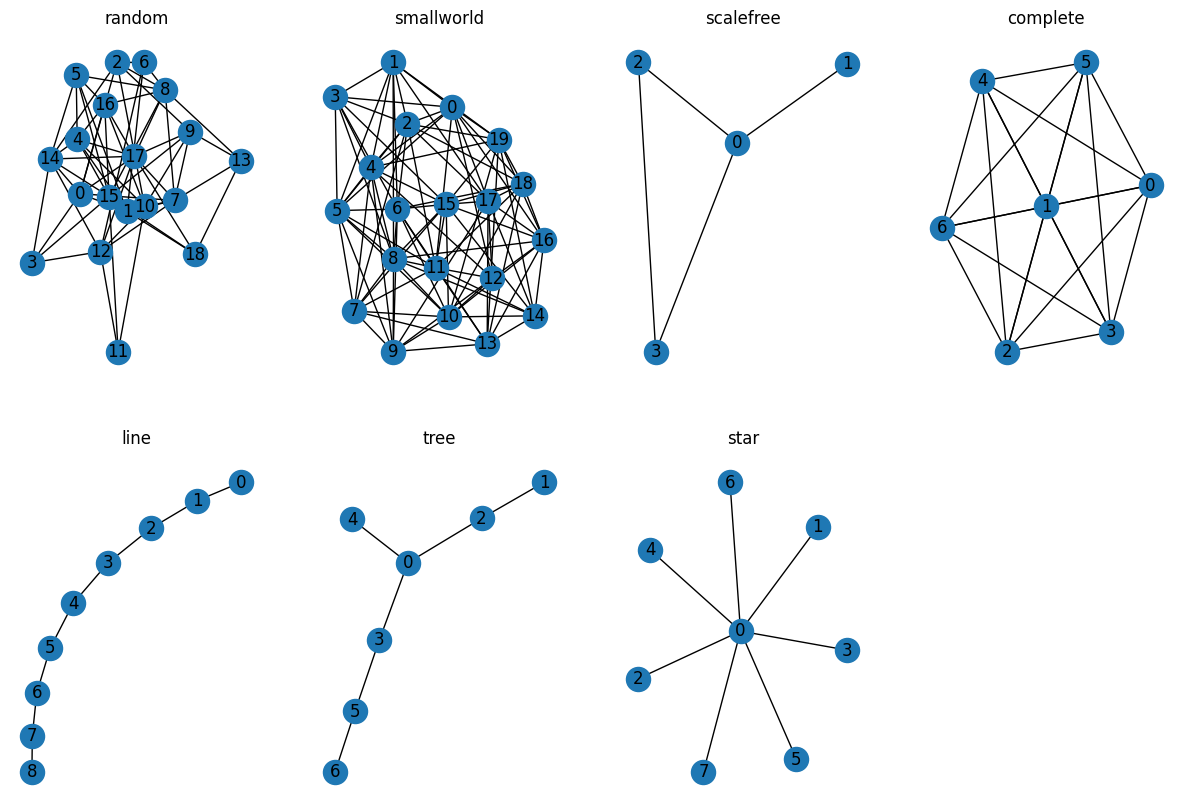
\includegraphics[width=0.6\textwidth]{images/42_data/example_graphs.png}
    \caption{Visualisierung von Graphen mit NetworkX und Matplotlib}
    \label{fig:example_graphs}
\end{figure}

Die Complete, Line-, Tree- und Star-Graphen unterscheiden sich schon bei der ersten Betrachtung stark.
Die Random-Graphen nach Erdős-Rényi und die Small-World-Graphen können auf den ersten Blick ähnlich aussehen, differieren jedoch in der topologischen Struktur, wie bereits in der Theorie erwähnt.

\subsection{Datenaufbereitung und Datenstruktur}

Die Graphen für die Arbeit werden mithilfe von Python und NetworkX erarbeitet \cite{hagberg_exploring_2008}.
Das erstellte Python-Dictionary mit den jeweiligen Graphen ist nachfolgend aufgeführt:

\begin{listing}[H]
    \begin{minted}
        [frame=lines,framesep=2mm,baselinestretch=1.2,bgcolor=LightGray,fontsize=\footnotesize,linenos]
        {python}    
dataset = {
    "random": [],
    "smallworld": [],
    "scalefree": [],
    "complete": [],
    "line": [],
    "tree": [],
    "star": [],
}
    \end{minted}
    \caption{Datenstruktur für die Testdaten}
\end{listing}

In einem nächsten Schritt werden die erstellten Graphen ihrer Klasse zugewiesen, was auch als \emph{Labeling} bezeichnet werden kann. Das Label der Graphen ist der Key des Dictionary.
Diese Labels werden für die spätere Klassifikationsaufgabe verwendet.